\documentclass{article}

\usepackage[%
    left=0.5in,%
    right=0.5in,%
    top=0.5in,%
    bottom=0.5in,%
]{geometry}%
\usepackage{minitoc}
\usepackage{multicol}
\usepackage{graphicx}
\usepackage{fixltx2e}
\usepackage{listings}
\usepackage{color}
\usepackage{hyperref}
    \hypersetup{ colorlinks = true, linkcolor = blue }
\usepackage{blindtext}
\definecolor{lightgray}{gray}{0.9}
\graphicspath{ {./} }

\newcommand{\inlinecode}[2]{\colorbox{lightgray}{\lstinline
[language=#1]$#2$}}
\newcommand{\worddef}[1]{\hyperref[sec:reference]{\textit{#1}}}

\begin{document}

\tableofcontents

\newpage

\section{Limitations of reactive architectures}
\begin{itemize}
  \item there are many things agents with reactive architectures can’t do:
  \begin{itemize}
    \item they can’t \textbf{represent or reason} about hypothetical objects and times;
    \item they don’t do well in domains where plausible actions \textbf{can’t be ignored or undone} if they prove to be unwise;
    \item it is difficult for purely reactive agents to \textbf{organise their own activities} over time or to coordinate their behaviour with that of other agents in a non-trivial way 
  \end{itemize}
  \item it’s difficult to get intelligent behaviour from a purely reactive agent
\end{itemize}

\section{Deliberation}
\begin{itemize}
  \item deliberation is the explicit consideration of \textbf{alternative courses of action} 
  \item deliberation involves \textbf{generating} alternatives and \textbf{choosing} an alternative 
  \item an agent can deliberate about:
  \begin{itemize}
    \item \textbf{means}: how to achieve a goal (this lecture)
    \item \textbf{ends}: whether to achieve (intend) a goal
  \end{itemize}
  \item \textbf{Examples}: deliberating about means
  \begin{itemize}
    \item problem solving (search) 
    \item planning 
    \item scheduling 
    \item theorem proving 
    \item constraint satisfaction
  \end{itemize}
\end{itemize}

\section{Deliberation architecture}
\begin{center}
  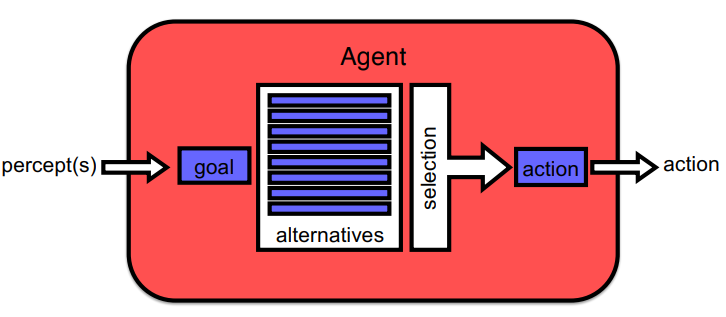
\includegraphics[scale=0.5]{deliberative_actor.png}
\end{center}

\subsection{Means}
\begin{itemize}
  \item in a deliberative architecture, percepts (or communication) \textbf{give rise to goals} (representations of a state to be achieved) and representations of the \textbf{current state of the world}
  \item the agent deliberates about how to achieve the goal
  \begin{itemize}
    \item deliberation involves (usually systematic) \textbf{exploration of alternative courses of action}
    \item a deliberative architecture typically includes automatic generation and comparison of alternatives
  \end{itemize}
  \item result of deliberation is a \textbf{representation of the action(s) to be performed}
\end{itemize}

\subsection{The role of representations}
\begin{itemize}
  \item deliberation involves the manipulation \textbf{of a model} of the world and possible courses of action, rather than the world itself 
  \item requires the ability to represent actions and derive the consequences of actions \textbf{without actually performing them}, e.g.:
  \begin{itemize}
    \item by remembering their effects in previous, similar situations
    \item by reference to a causal model of the world
  \end{itemize}
\end{itemize}

\subsection{Counterfactual representations}
\begin{itemize}
  \item to represent desired states and the consequences of actions:
  \begin{itemize}
    \item some states of the agent must be counterfactual in the sense of \textbf{referring to hypothetical future states} (goals) or as yet unexecuted actions (plans)
    \item some of the basic operations of the architecture should generate such counterfactual states
    \item such states must be influential in the choice of actions
  \end{itemize}
  \item to represent hypothetical situations, a deliberative agent requires representations with \worddef{compositional semantics}
\end{itemize}

\subsection{Advantages of deliberation}
\begin{itemize}
  \item useful when the \textbf{penalty} for incorrect actions is high, e.g., when the environment is hazardous 
  \item allows us to code a general procedure for finding a solution to a class of problems
  \begin{itemize}
    \item may be better than reactive systems at \textbf{coping with novel problems}
    \item we may be able to get a correct or even an optimal answer, e.g., decision theoretic approaches
  \end{itemize}
\end{itemize}

\section{TSP algorithms}
\begin{itemize}
  \item many TSP algorithms use iterative refinement, i.e., they require the representation of at least two alternative tours:
  \begin{itemize}
    \item the \textit{current best tour} (best known route)
    \item the \textit{candidate tour} (often a modification of the current best tour)
  \end{itemize}
  \item iterative algorithms typically stop when no modification of the current best tour \textbf{has lower cost} or when there has been \textbf{no improvement} for n iterations 
  \item agent then executes the steps in the current best tour
\end{itemize}

\subsection{Shakey}
\begin{flushleft}
Look at lecture notes \href{https://moodle.nottingham.ac.uk/pluginfile.php/4573264/mod_resource/content/6/05%20Deliberative%20Architectures%20I.pdf}{here}
\end{flushleft}

\section{Planning}
\begin{itemize}
  \item the agent’s knowledge of the \textit{initial state} of the world is often \textbf{incomplete or mistaken }
  \item the world is continually changing and continues to change \textbf{while the agent is planning}
  \item actions don’t always have the intended effect—actions can fail or just have \textbf{unpredictable outcomes} 
  \item the agent may \textbf{make errors executing the plan} 
  \item the time available to find a solution may be \textbf{limited}
\end{itemize}

\subsection{Simplifying assumptions}
\begin{itemize}
  \item the agent has \textbf{perfect knowledge of the world}, including the location and properties of all the objects in the world 
  \item the world is \textbf{static}—i.e., it doesn’t change unless the agent changes it 
  \item the world is \textbf{deterministic}: we know in advance \textbf{the effect} of performing an action in the world and each action has a single outcome 
  \item plan execution is error-free and it doesn’t matter how long it takes the agent to find a plan
\end{itemize}

\subsection{Classical planning}
\begin{itemize}
  \item if we make these assumptions we get classical planning (production of a complete, totally ordered set of actions, which, when executed in a given initial situation, will achieve a goal)
  \item resulting sequence of actions will typically only work if the \textbf{simplifying assumptions hold} 
  \item implies some way of coping with inaccurate world models, nondeterministic actions, plan execution errors, etc
\end{itemize}

\subsection{STRIPS}
\begin{itemize}
  \item states are represented as conjunctions of (function-free) ground literals 
  \item goals are represented by conjunctions of literals, possibly containing existentially quantified variables 
  \item actions are represented by operators which specify
  \begin{itemize}
    \item the name of the action
    \item the precondition: a conjunction of positive literals specifying what must be true for the action to be applicable
    \item the postcondition: a conjunction of literals specifying how the situation changes when the operator is applied
  \end{itemize}
  \item for example, an operator which stacks one block on top of another in the blocks world could be specified as
  \begin{itemize}
    \item $[Clear(x), Clear(y)] STACK(x, y) [ On(x, y), ¬Clear(y) ]$
  \end{itemize}
  \item the precondition implicitly refers to the situation, s, immediately before the action, and the postcondition implicitly refers to the situation, s′, which results from performing the action 
  \item in s′ , all the positive literals in the postcondition hold, as do all the literals that held at s, except for those that are negative literals in the postcondition
\end{itemize}

\subsection{Regression planning}
\begin{itemize}
  \item one way to solve STRIPS problems is to \textbf{search backwards} from the goal in world (situation) space 
  \item operator preconditions become \textit{subgoals} - we stop when the operator preconditions are satisfied in the current state 
  \item searching backwards often \textbf{reduces} the branching factor 
  \item in typical problems the goal state has a small number of conjuncts, each of which is made true by a small number of operators, while there are many operators that can be applied in the initial state 
  \item resulting plan is a series of instantiated operators which, if applied in the initial state, result in the goal state
\end{itemize}

\pagebreak
\section*{Reference section} \label{sec:reference}
\begin{description}
	\item[compositional semantics] \hfill \\ The meaning of a phrase is determined by combining the meanings of its subphrases, using rules which are driven by the syntactic structure.
\end{description}
\end{document}
